%\documentclass{article}
%\usepackage{graphicx,subfigure}
%\begin{document}

\begin{figure}[h]
  \centering
   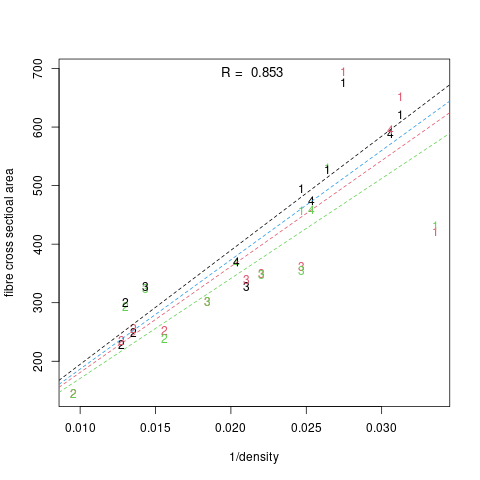
\includegraphics[width=1.1\textwidth]{SDP/sdpArecN.png}
  \caption{Plot of reciprocal density against cross sectional area of tenth staole segment for data from Jackson and Downes (1979)~\cite{jack:79}. Regression lines are through the origin. Black is D+ Line, red is D- Line. Green  is L+ Line. Blue is L- Line} 
  \label{fig:sdpArecN}
\end{figure}

%\end{document}

